% Created 2020-01-16 Thu 16:38
% Intended LaTeX compiler: pdflatex
\documentclass{beamer}
\usepackage[utf8]{inputenc}
\usepackage[T1]{fontenc}
\usepackage{graphicx}
\usepackage{grffile}
\usepackage{longtable}
\usepackage{wrapfig}
\usepackage{rotating}
\usepackage[normalem]{ulem}
\usepackage{amsmath}
\usepackage{textcomp}
\usepackage{amssymb}
\usepackage{capt-of}
\usepackage{hyperref}
\usetheme{UoB}
\author{Mark Blyth}
\date{\textit{[2020-01-20 Mon]}}
\title{A Rinzel-esque bifurcation analysis of some bursting models}
\hypersetup{
 pdfauthor={Mark Blyth},
 pdftitle={A Rinzel-esque bifurcation analysis of some bursting models},
 pdfkeywords={},
 pdfsubject={},
 pdfcreator={Emacs 26.3 (Org mode 9.1.9)}, 
 pdflang={English}}
\begin{document}

\maketitle

\section{Background}
\label{sec:orgcd36d14}
\begin{frame}[label={sec:org0e1c8e9}]{Week's goal}
\begin{itemize}
\item Focus on bifurcation analysis of Krassy's system
\item Use it as an opportunity to learn about continuation software
\item Once I know enough about any one software, write up about it for the paper
\end{itemize}
\end{frame}
\begin{frame}[label={sec:org67d2b96}]{Week's activities}
\begin{itemize}
\item Attempted to read some pure-maths papers about bifurcations of Krassy's cubic Lienard system
\begin{itemize}
\item No success
\end{itemize}
\item Attempted instead to do a bifurcation analysis on the cubic Lienard system 
\begin{itemize}
\item No success
\end{itemize}
\item Tried a Rinzel-esque fast-subsystem bifurcation analysis on the HR model (simpler, therefore easier)
\begin{itemize}
\item No success in XPP
\item Some success in MATCONT
\end{itemize}
\item Went back to Krassy's neuron model again, with newfound MATCONT skills
\begin{itemize}
\item Slightly more success?
\end{itemize}
\end{itemize}
\end{frame}

\section{Papers}
\label{sec:org679cd97}
\begin{frame}[label={sec:org4479f9b}]{Global study of a family of cubic Lienard equations}
\begin{itemize}
\item Krassy's model uses a cubic Lienard equation as the fast subsystem
\item This paper derives the global bifurcation diagram of that system
\item It's hard.
\end{itemize}

\vfill
\emph{Khibnik, Alexander I., Bernd Krauskopf, and Christiane Rousseau. "Global study of a family of cubic Liénard equations." Nonlinearity 11.6 (1998): 1505.}
\end{frame}

\begin{frame}[label={sec:org279ac95}]{Fast subsystem bifurcations in a slowly varying lienard sysetem exhibiting bursting}
\begin{itemize}
\item Krassy's model uses a cubic Lienard equation as the fast subsystem
\item This paper performs various rigorous analyses on that system
\item It's hard.
\end{itemize}

\vfill

\emph{Pernarowski, Mark. "Fast subsystem bifurcations in a slowly varying Lienard system exhibiting bursting." SIAM Journal on Applied Mathematics 54.3 (1994): 814-832.}
\end{frame}

\section{HR Bifurcations}
\label{sec:org9700964}
\begin{frame}[label={sec:orgcb52265}]{A first attempt at bifurcation diagrams}
\begin{itemize}
\item Tried to do a bifurcation analysis of Krassy's system
\begin{itemize}
\item No success
\end{itemize}
\item Decided instead to try a Rinzel-esque analysis of the HR system
\begin{itemize}
\item Simple system capable of exhibiting bursting
\item Some success
\end{itemize}
\end{itemize}
\end{frame}

\begin{frame}[label={sec:orgf0abdbb}]{The Hindmarsh-Rose model}
A very popular bursting model, given by

\begin{align}
\frac{\mathrm d x}{\mathrm d t} &= y - ax^3 +bx^2-z+I~,\\
\frac{\mathrm d y}{\mathrm d t} &= c - dx^2 -y~,\\
\frac{\mathrm d z}{\mathrm d t} &= r\left[s(x-x_R)-z\right]~.
\end{align}

\vfill
\emph{Hindmarsh, James L., and R. M. Rose. "A model of neuronal bursting using three coupled first order differential equations." Proceedings of the Royal society of London. Series B. Biological sciences 221.1222 (1984): 87-102.}
\end{frame}

\begin{frame}[label={sec:orgbc6eeb9}]{HR Bifurcations}
\begin{itemize}
\item \(b\) influences whether or not the cell bursts, and \(z\) is the slow subsystem variable.
\item Idea: codim-2 bifurcation analysis of the fast subsystem, in terms of \((b,z)\)
\begin{itemize}
\item Goal: find the bifurcations that start and end the hysteresis loop, in the same way as Rinzel classifies bursters
\item Approach it with minimal knowlege of the system, so that I'm learning, rather than copying papers!
\end{itemize}
\end{itemize}
\end{frame}

\begin{frame}[label={sec:orgf48c800}]{HR Bifurcations}
\begin{center}
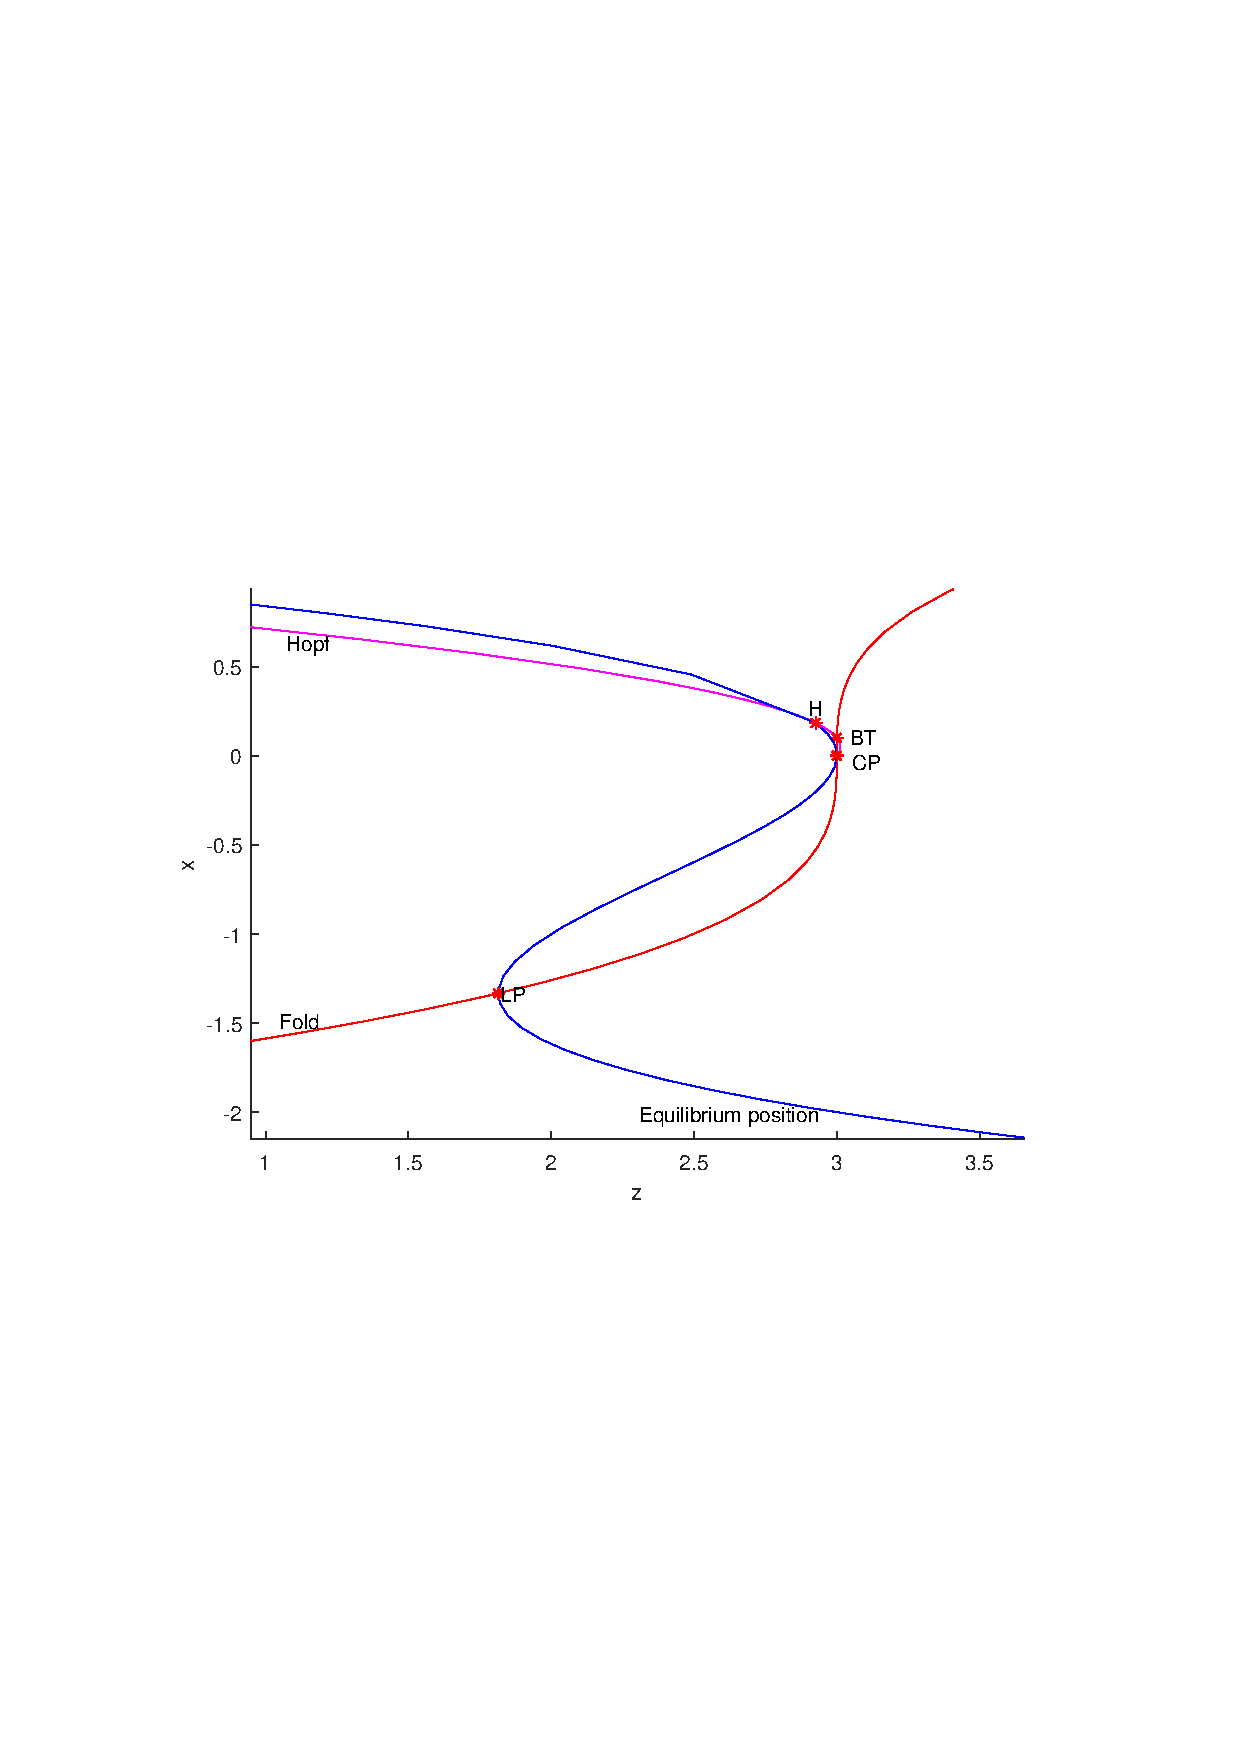
\includegraphics[trim={3cm 9cm 4cm 10cm}, clip,height=.9\textheight]{HRzbBif2.pdf}
\end{center}
\end{frame}

\begin{frame}[label={sec:org6cf1500}]{HR Bifurcations}
\begin{center}
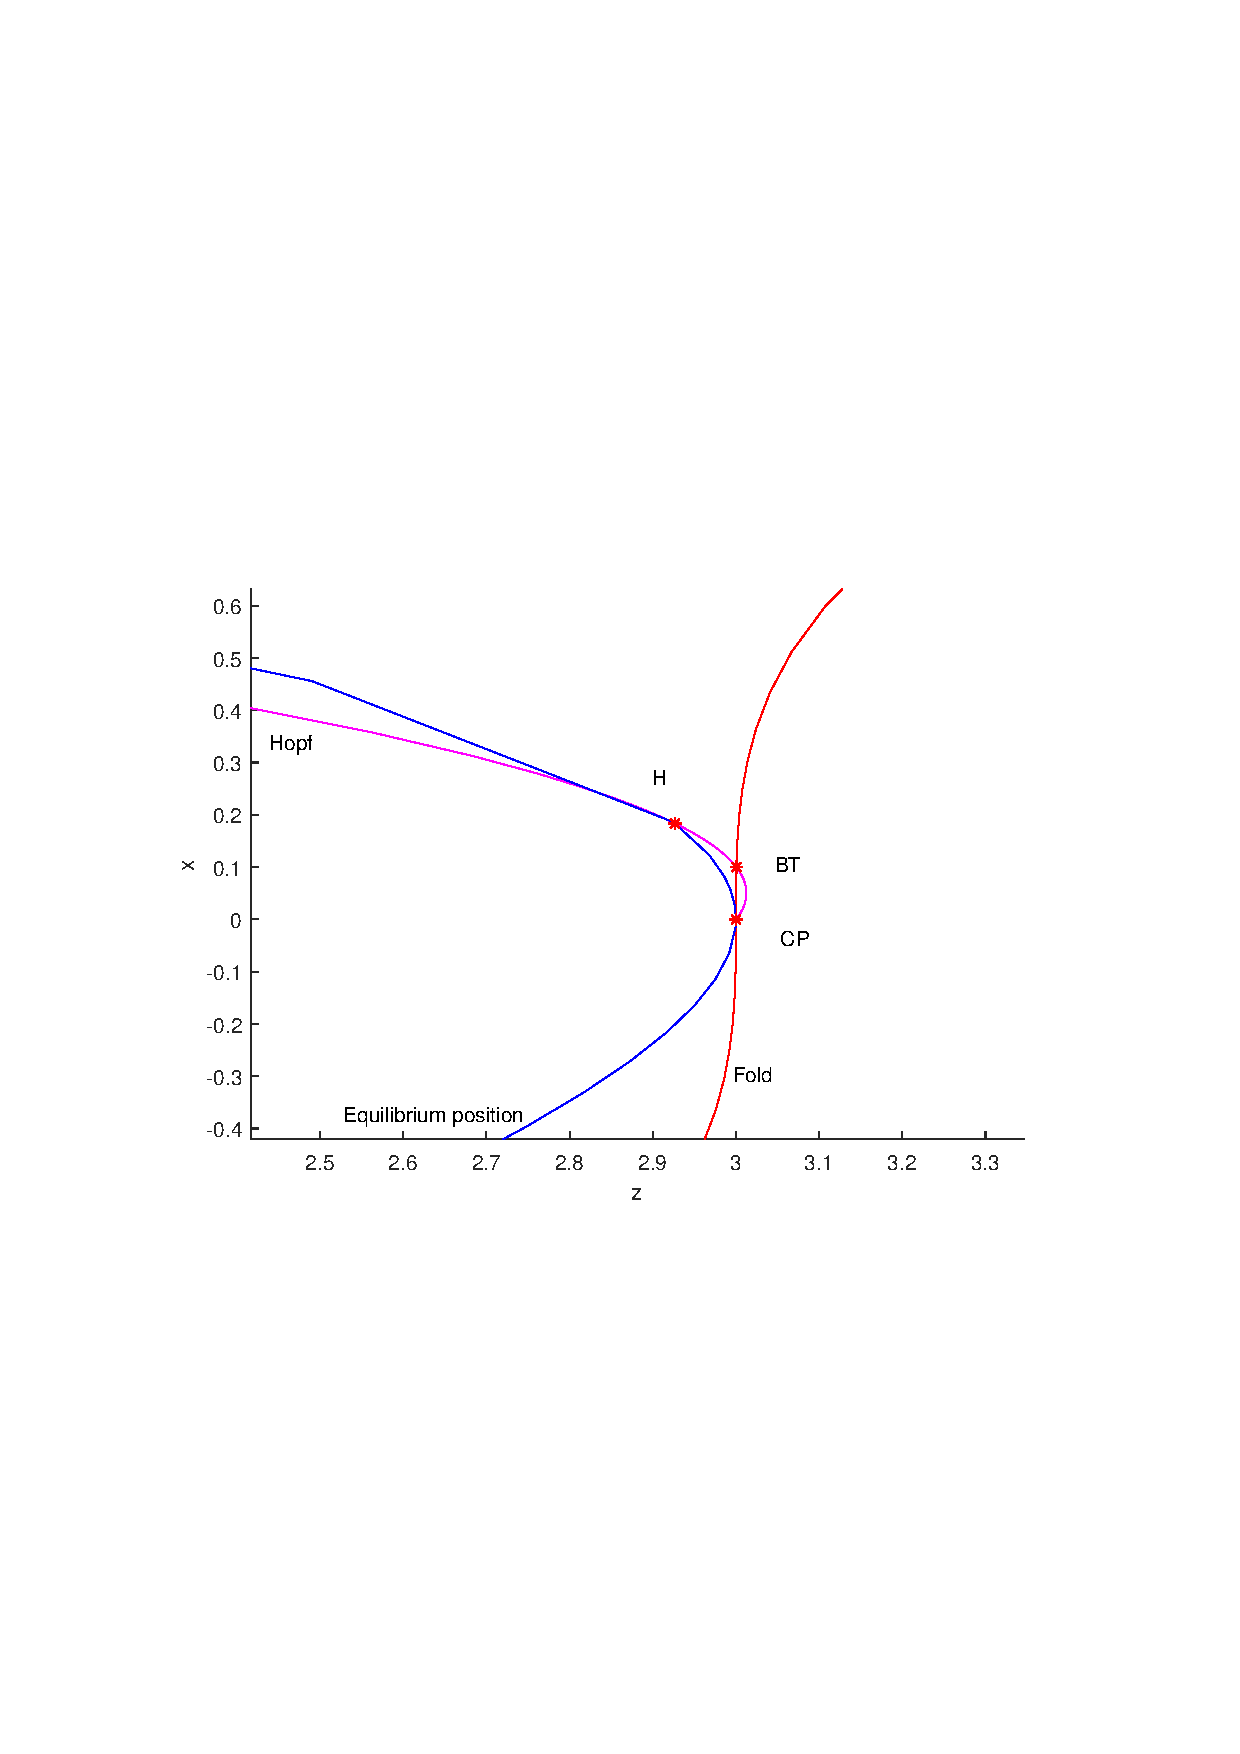
\includegraphics[trim={3cm 9cm 4cm 10cm}, clip,height=.9\textheight]{HRzbBif3.pdf}
\end{center}
\end{frame}

\begin{frame}[label={sec:orgb5779e5}]{HR Bifurcations}
\begin{center}
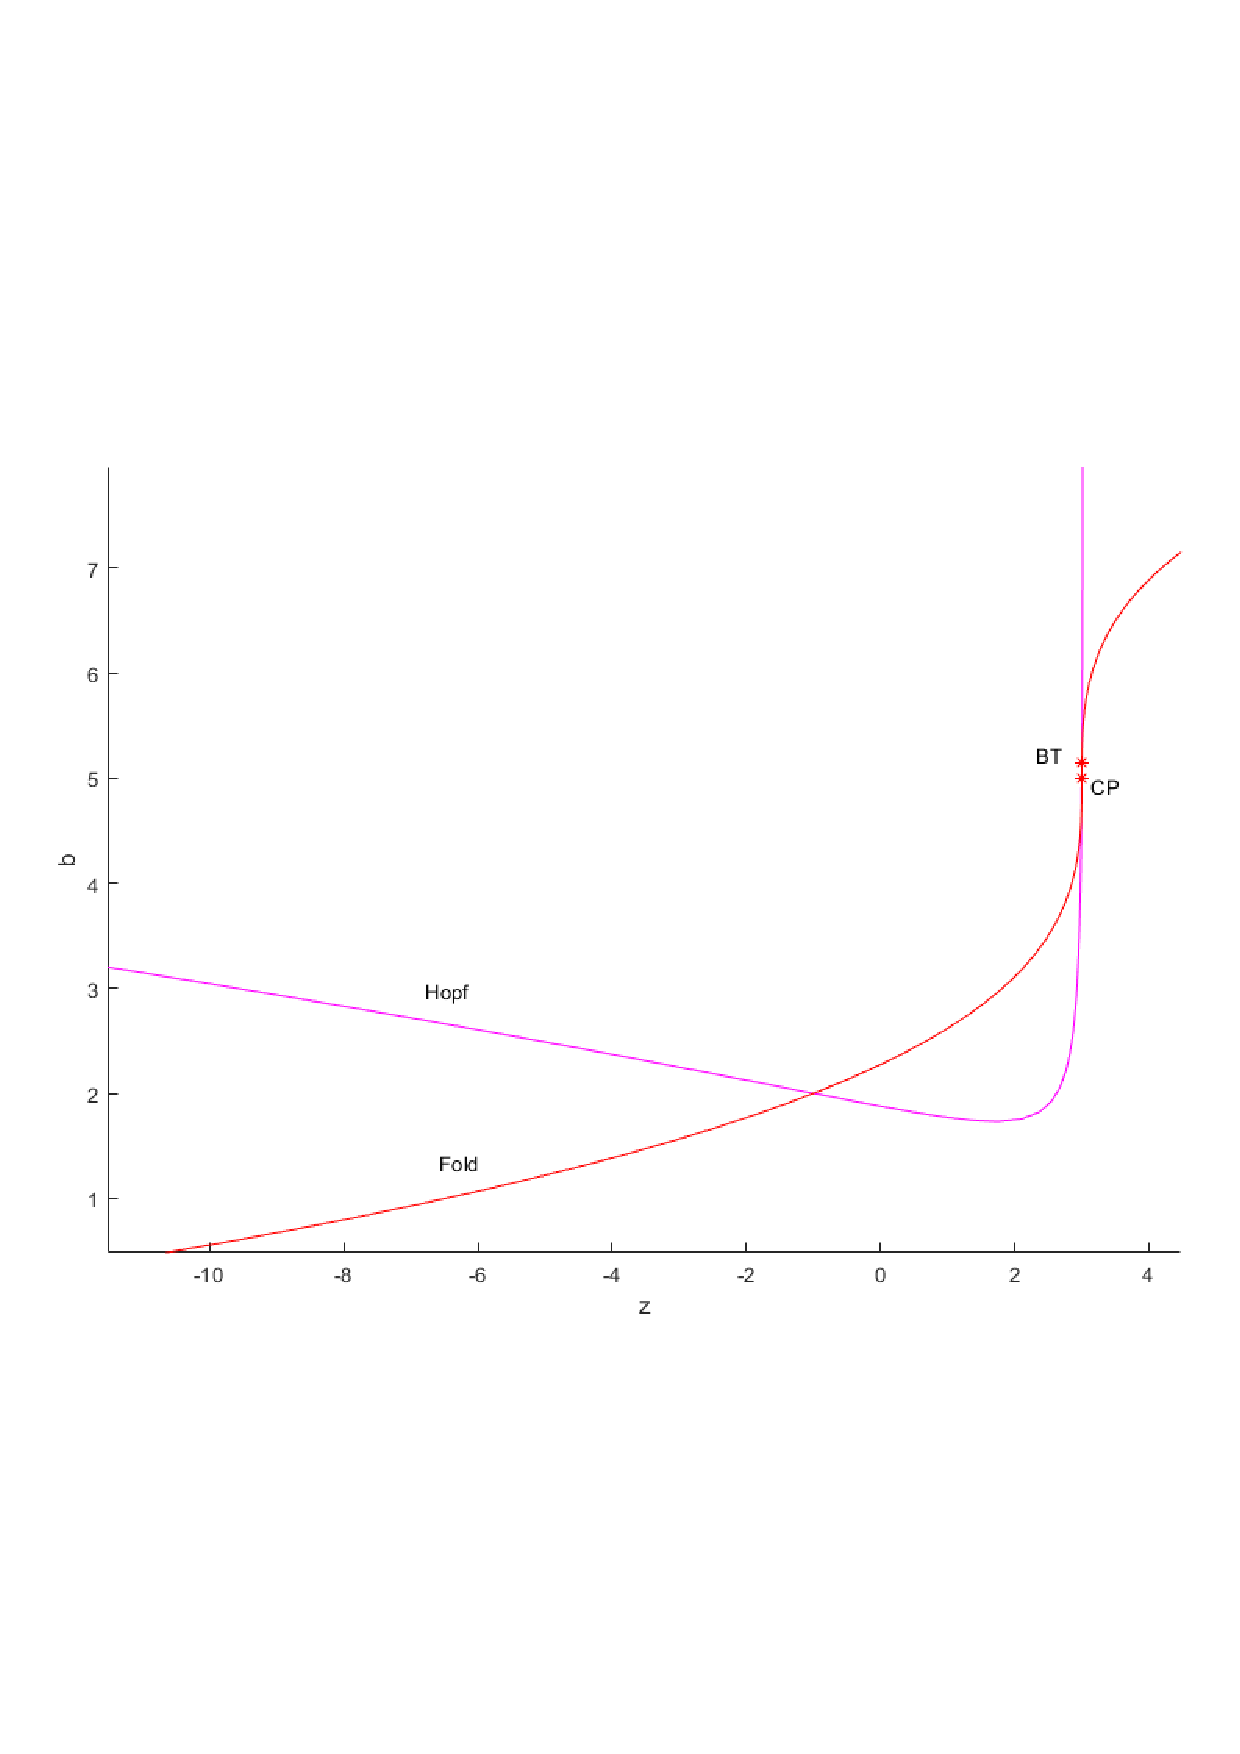
\includegraphics[trim={1cm 7cm 1cm 8cm}, clip,height=.9\textheight]{HRzbBif.pdf}
\end{center}
\end{frame}

\begin{frame}[label={sec:org0e83b17}]{HR Bifurcations}
\begin{itemize}
\item Taking \(b=3\) (Wikipedia default value) gives a codim-2 Fold-Hopf burster
\item I haven't dug into the literature to see if this is right (I don't think it is)
\end{itemize}
\end{frame}

\begin{frame}[label={sec:orgbc548b6}]{HR Bifurcations}
\begin{center}
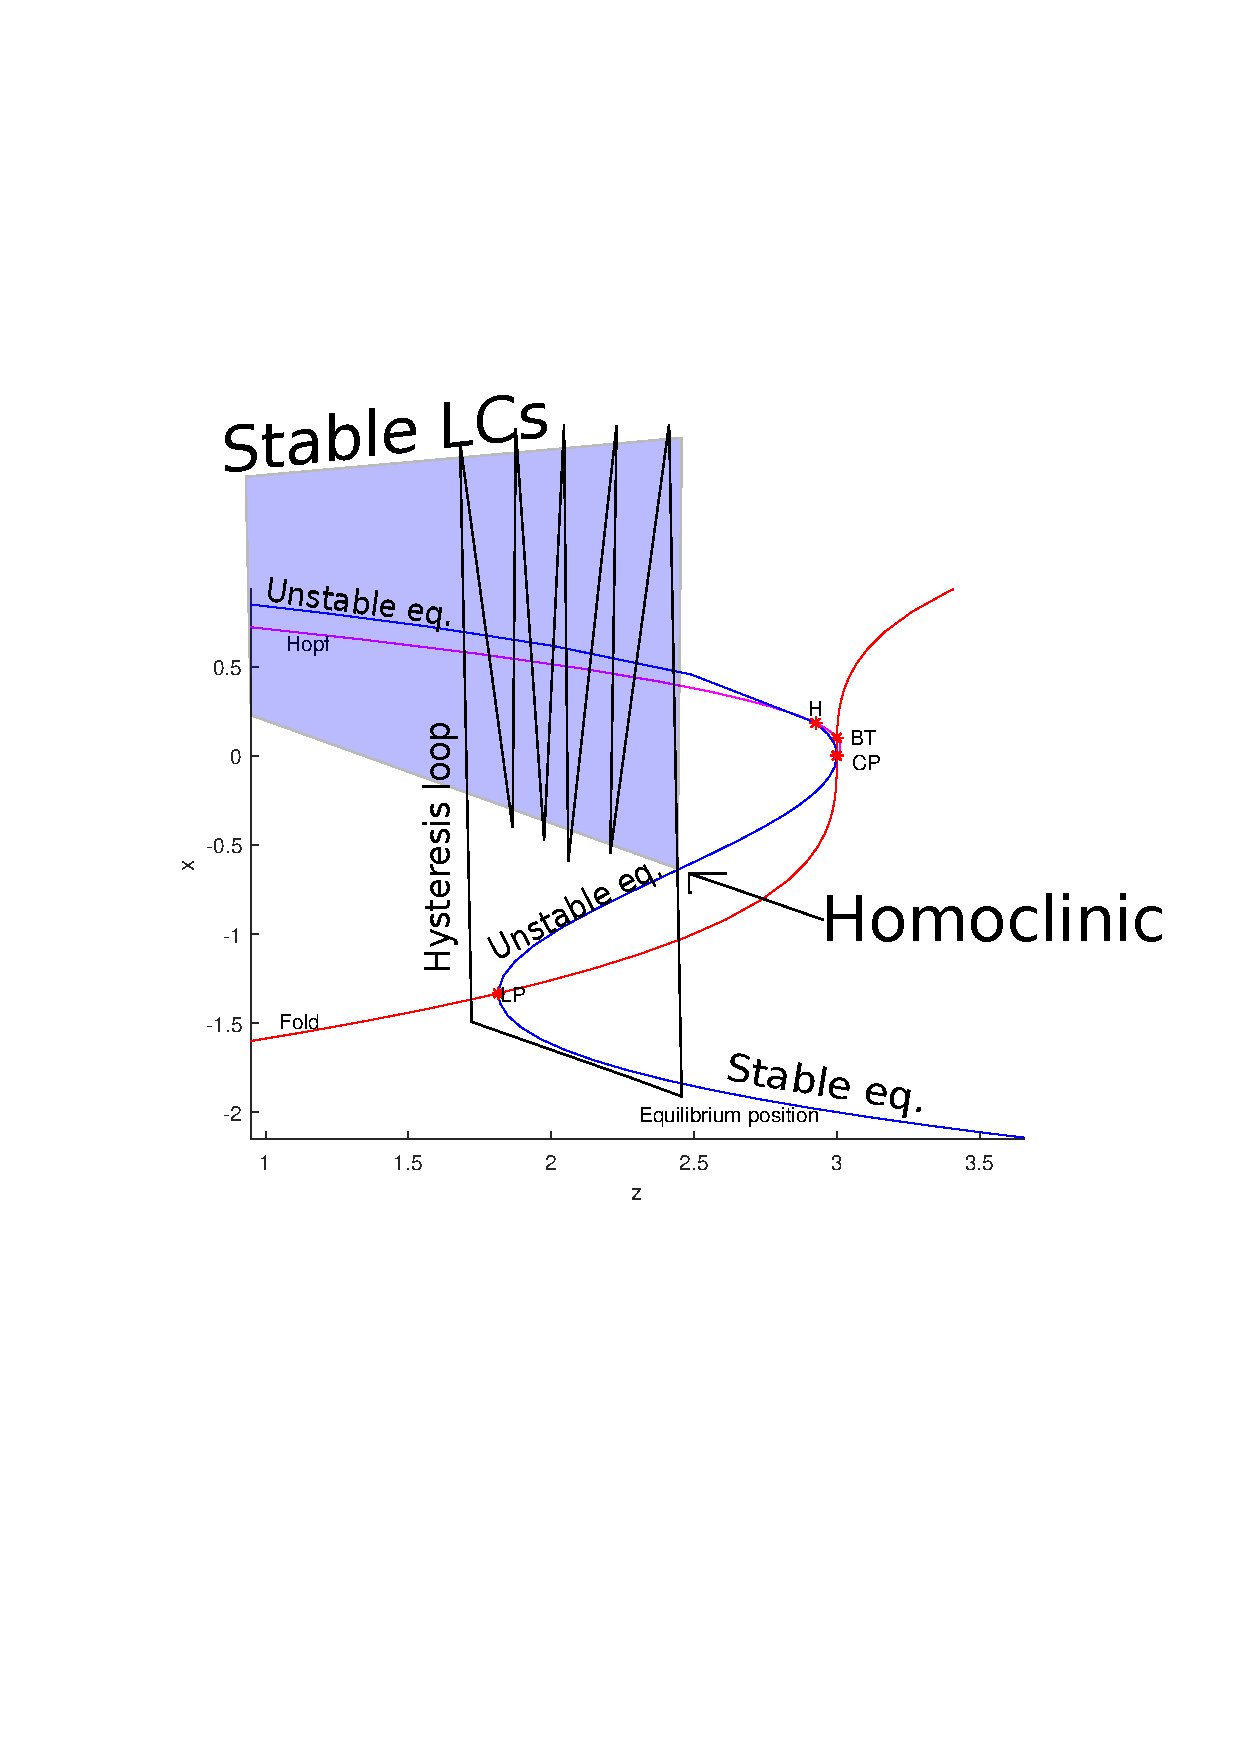
\includegraphics[trim={3cm 9cm 0cm 5cm}, clip,height=.9\textheight]{HRzbBif2 (copy 1).pdf}
\end{center}
\end{frame}

\section{Krassy's model (attempt 2)}
\label{sec:org52a1b16}
\begin{frame}[label={sec:orgeb49717}]{Cubic Lienard system}
\begin{columns}
\begin{column}{0.4\columnwidth}
\begin{itemize}
\item Hold \(b\), \(\nu\) fixed
\item Sweep \(\mu_1,\mu_2\)
\item Inspired by stuff I didn't understand in Krassy's paper
\item Some similarities to the bifurcation diagrams in the paper\ldots{}
\end{itemize}
\end{column}

\begin{column}{0.6\columnwidth}
\begin{center}
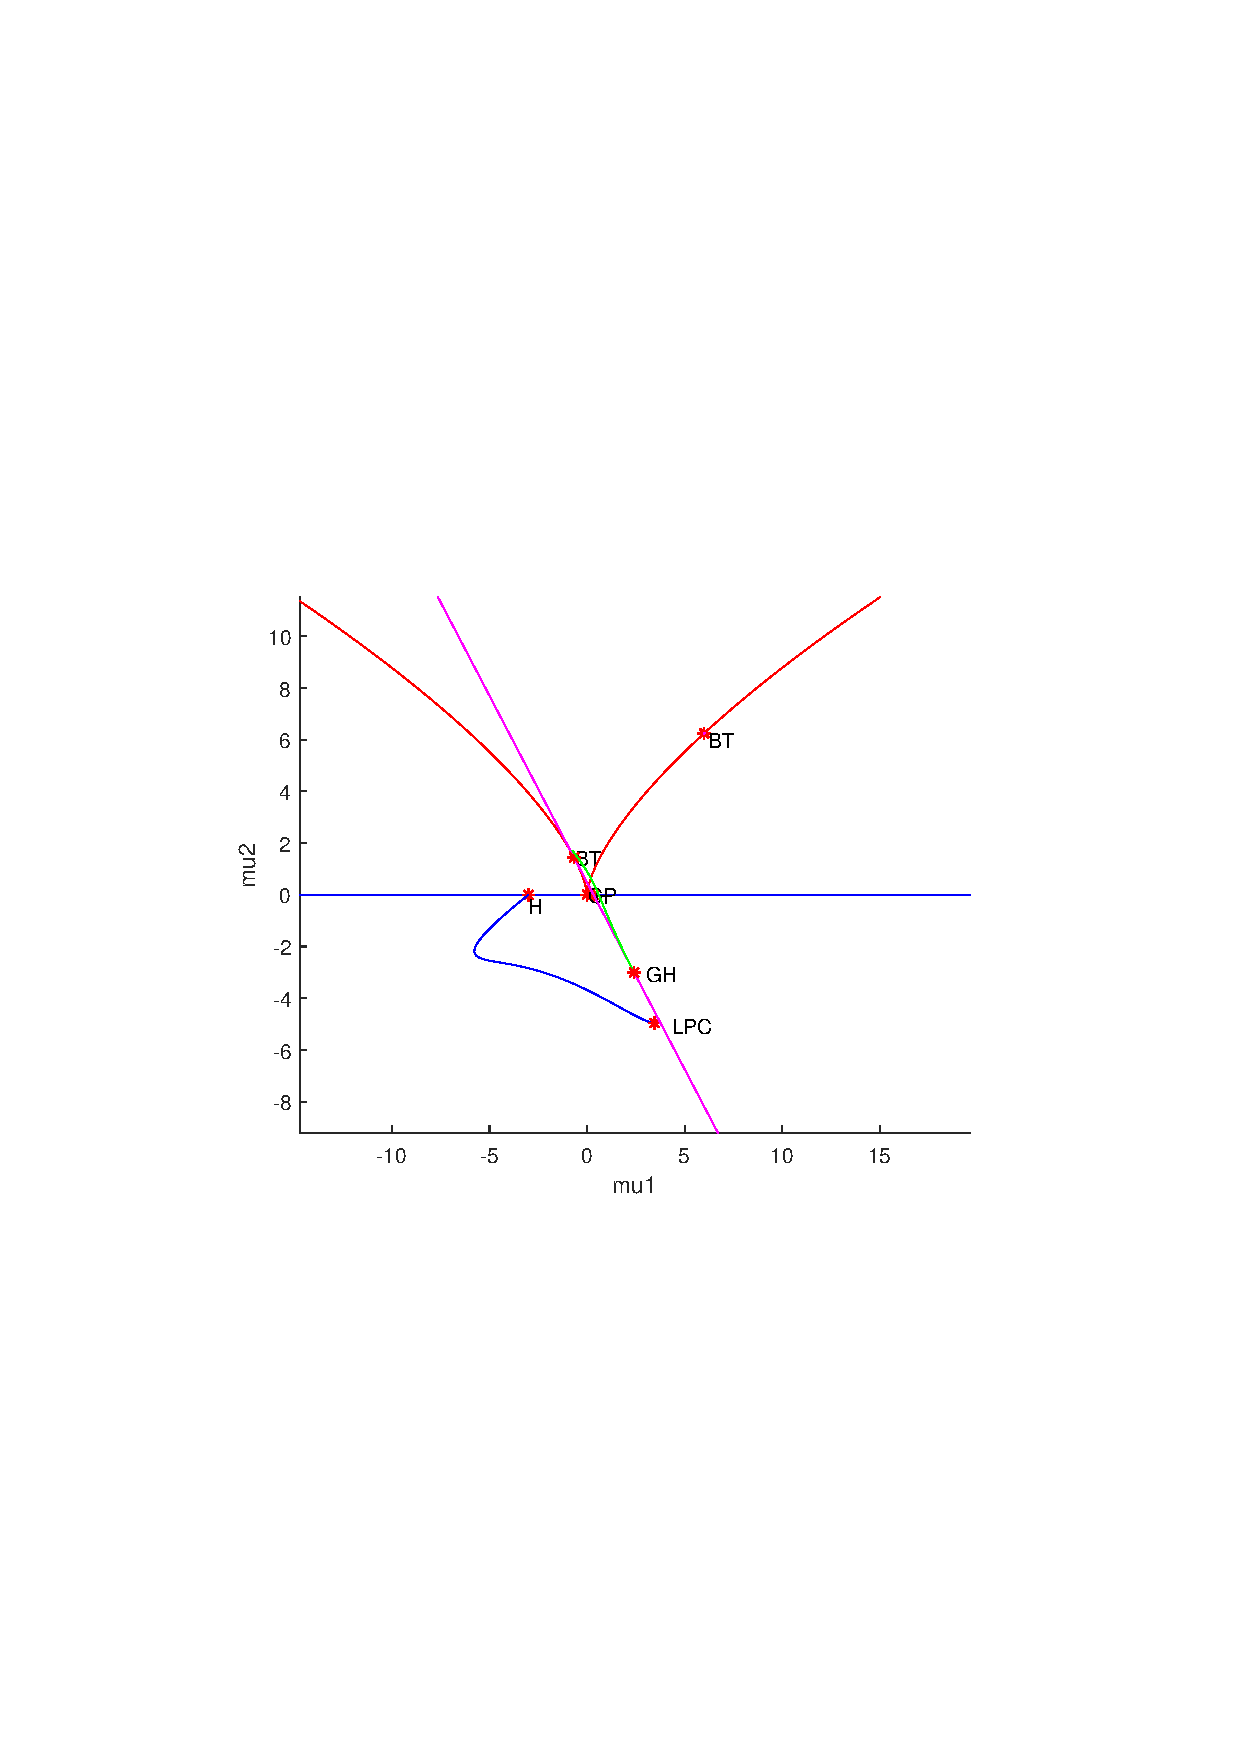
\includegraphics[trim={4cm 8cm 3cm 10cm}, clip,width=\textwidth]{krassy.pdf}
\end{center}
\end{column}
\end{columns}
\end{frame}

\begin{frame}[label={sec:orgecbea0e}]{Attempt 2}
\begin{columns}
\begin{column}{0.4\columnwidth}
\begin{itemize}
\item Tried to recreate a bifurcation diagram from Krassy's paper
\item Took their parameter values, mostly succeeded
\item Can't continue Homoclinics from Bogdanov-Takens points
\item Strange blue line?
\end{itemize}
\end{column}
\begin{column}{0.6\columnwidth}
\begin{center}
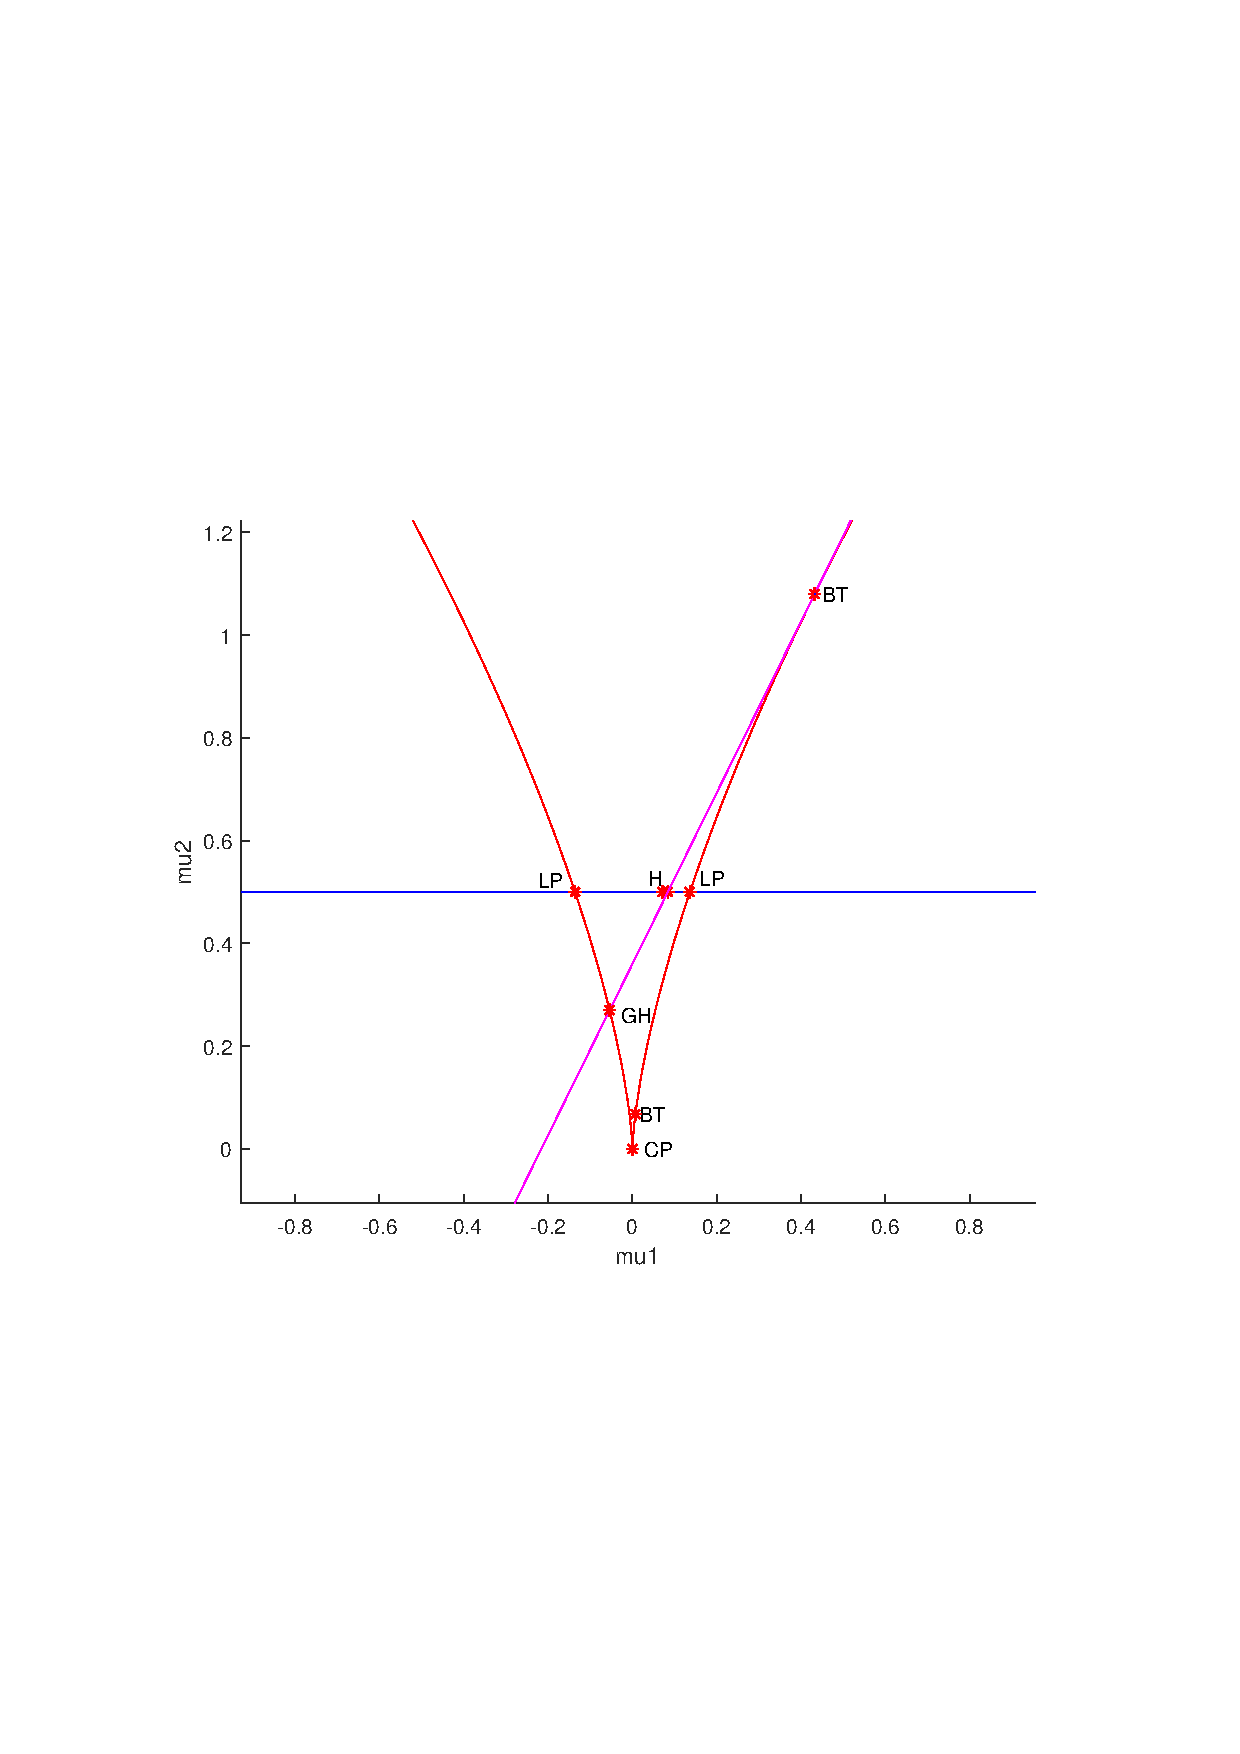
\includegraphics[trim={4cm 8cm 3cm 9cm}, clip,height=.8\textheight]{krassV2.pdf}
\end{center}
\end{column}
\end{columns}
\end{frame}

\begin{frame}[label={sec:org9f2aa25}]{Attempt 2 - mostly right}
\begin{columns}
\begin{column}{0.4\columnwidth}
\begin{center}
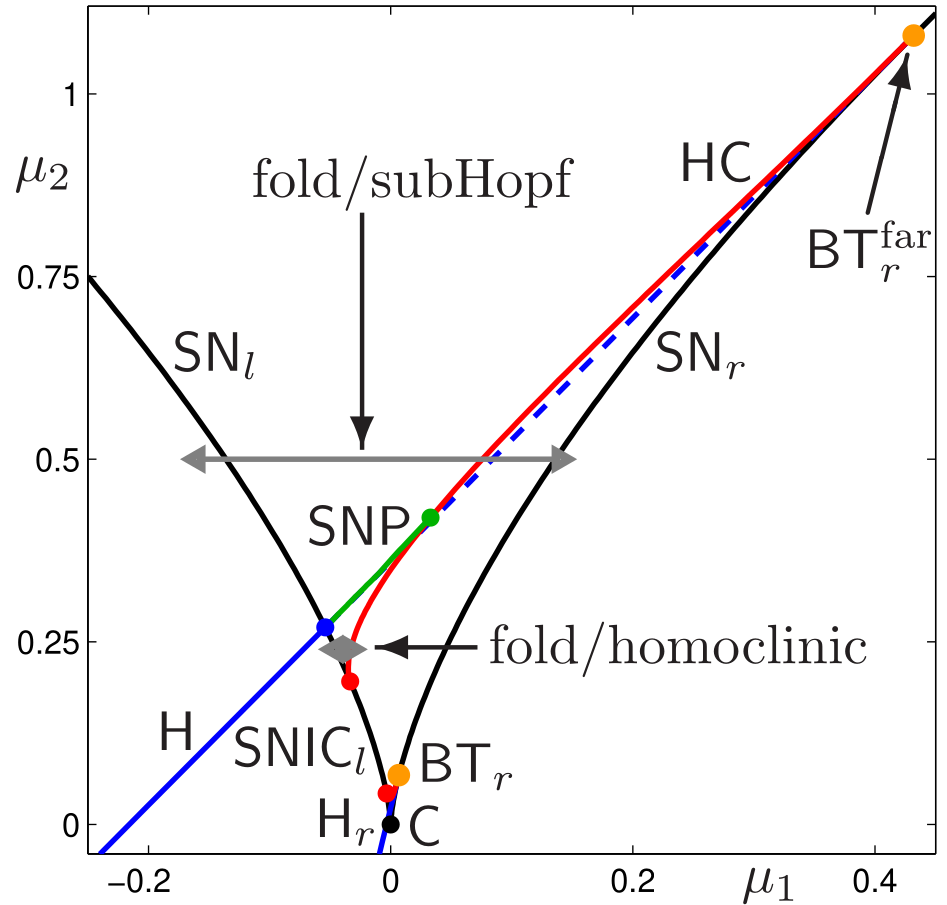
\includegraphics[width=\textwidth]{original.png}
\end{center}
\end{column}

\begin{column}{0.6\columnwidth}
\begin{center}
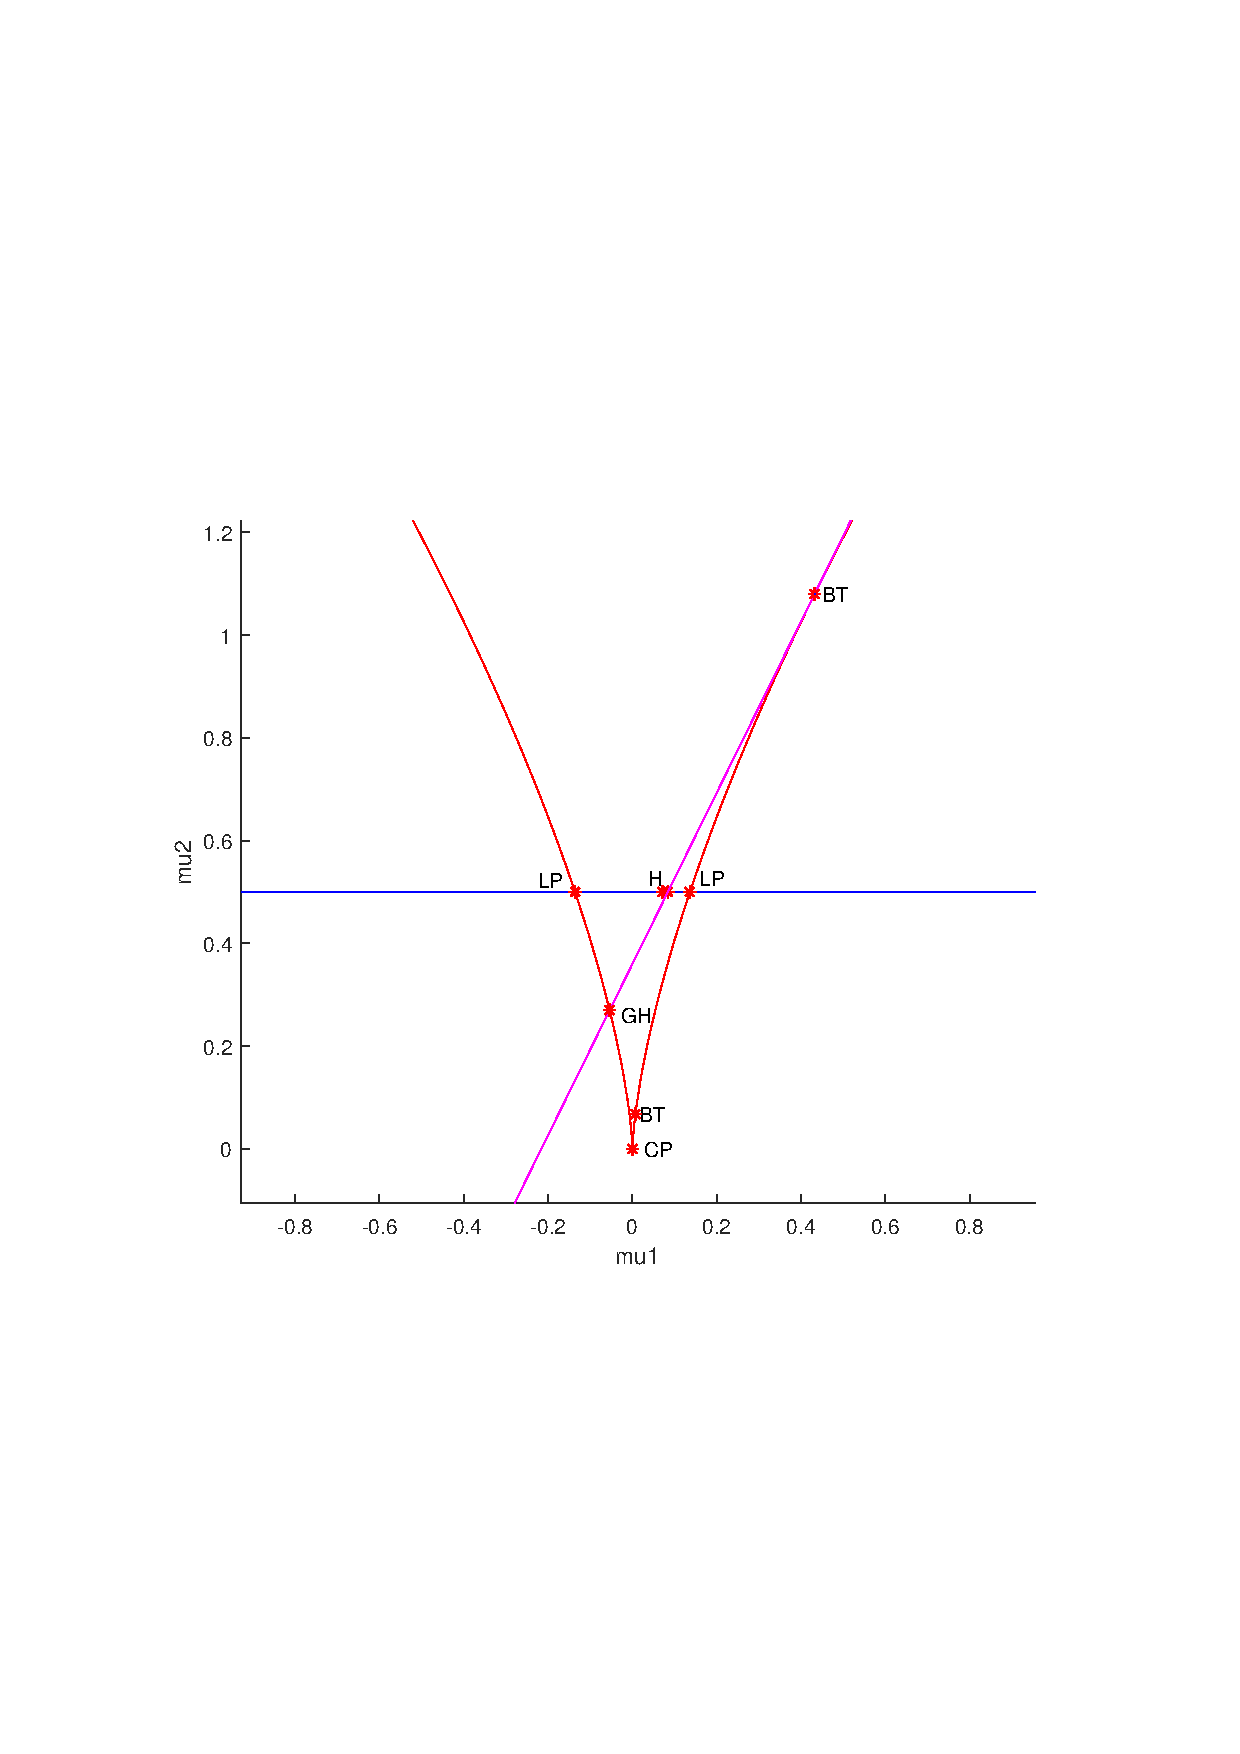
\includegraphics[trim={4cm 8cm 3cm 9cm}, clip,height=.8\textheight]{krassV2.pdf}
\end{center}
\end{column}
\end{columns}
\end{frame}
\section{AUTO}
\label{sec:orgbe31537}

\begin{frame}[label={sec:org0c450eb}]{HR model in AUTO}
\begin{center}
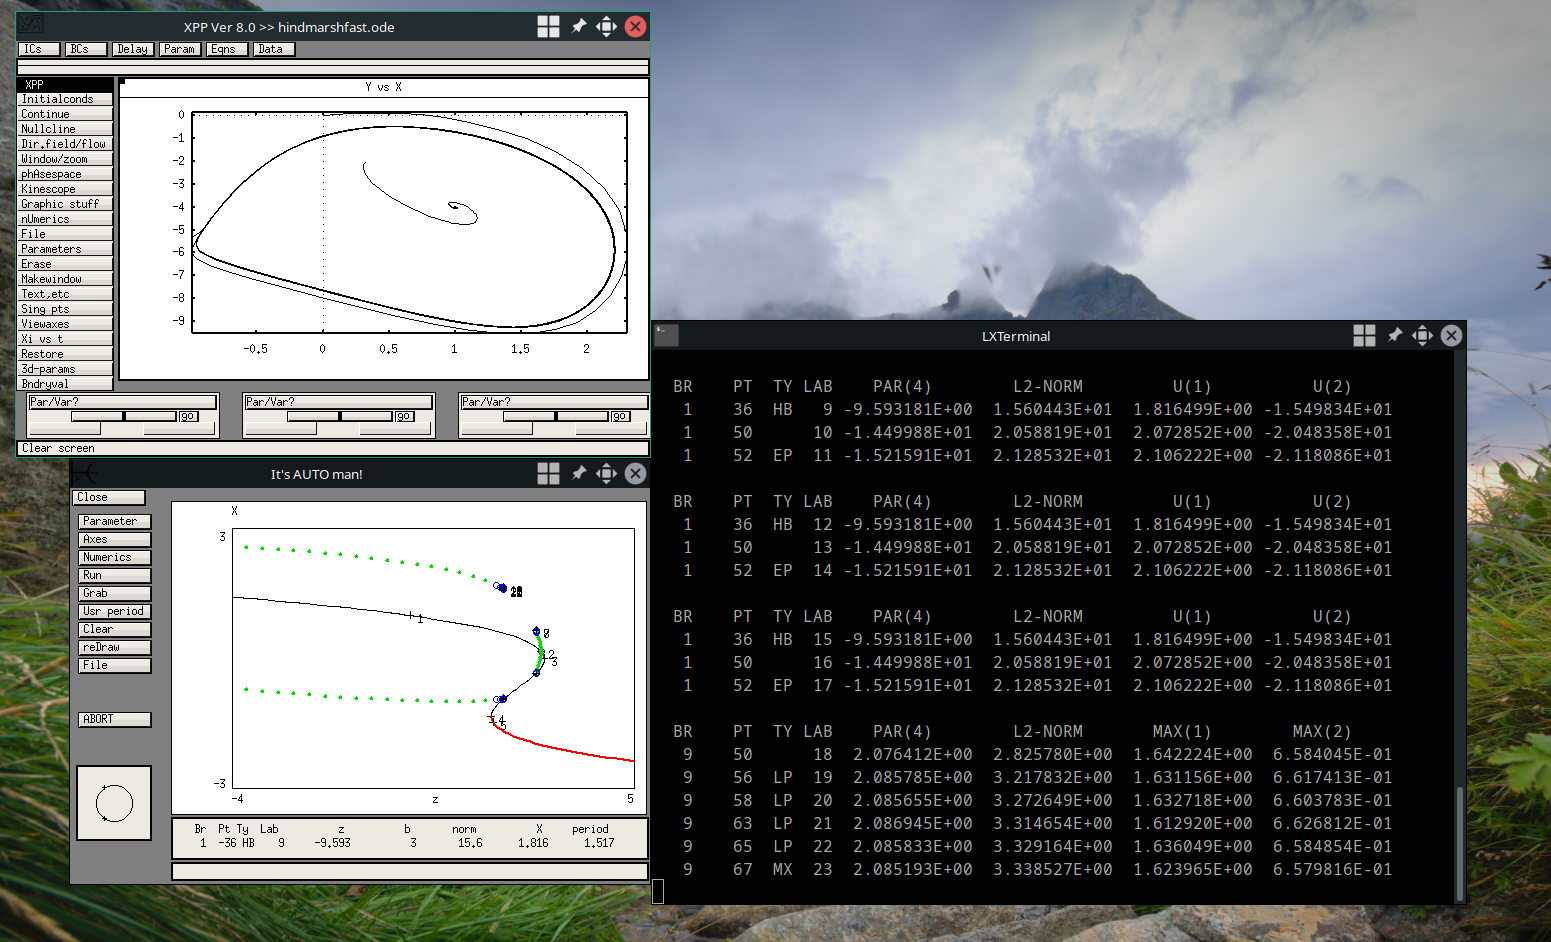
\includegraphics[height=.9\textheight]{auto2.png}
\end{center}
\end{frame}

\begin{frame}[label={sec:orgd7be187}]{HR Bifurcations in MATCONT (again)}
\begin{center}
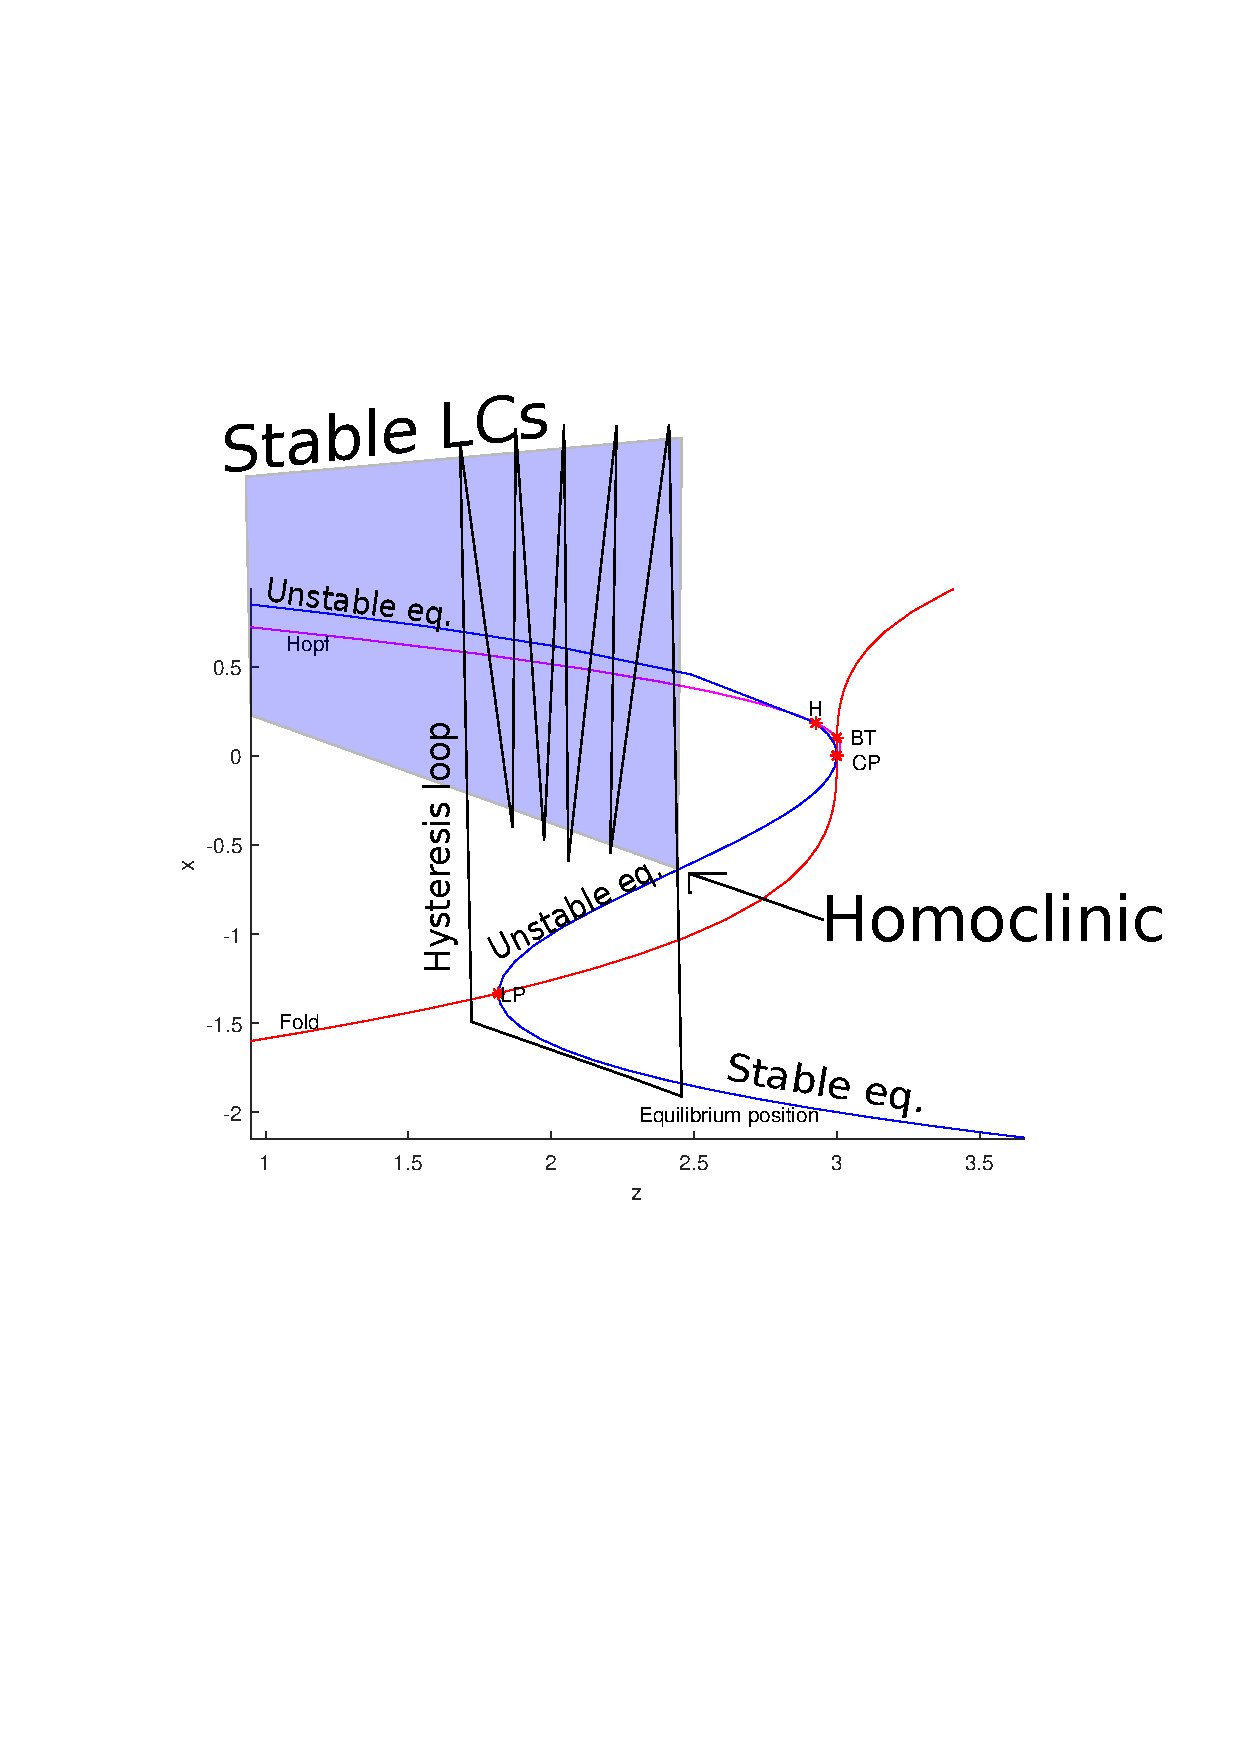
\includegraphics[trim={3cm 9cm 0cm 5cm}, clip,height=.9\textheight]{HRzbBif2 (copy 1).pdf}
\end{center}
\end{frame}

\begin{frame}[label={sec:org2a6a545}]{HR model in AUTO}
\begin{center}
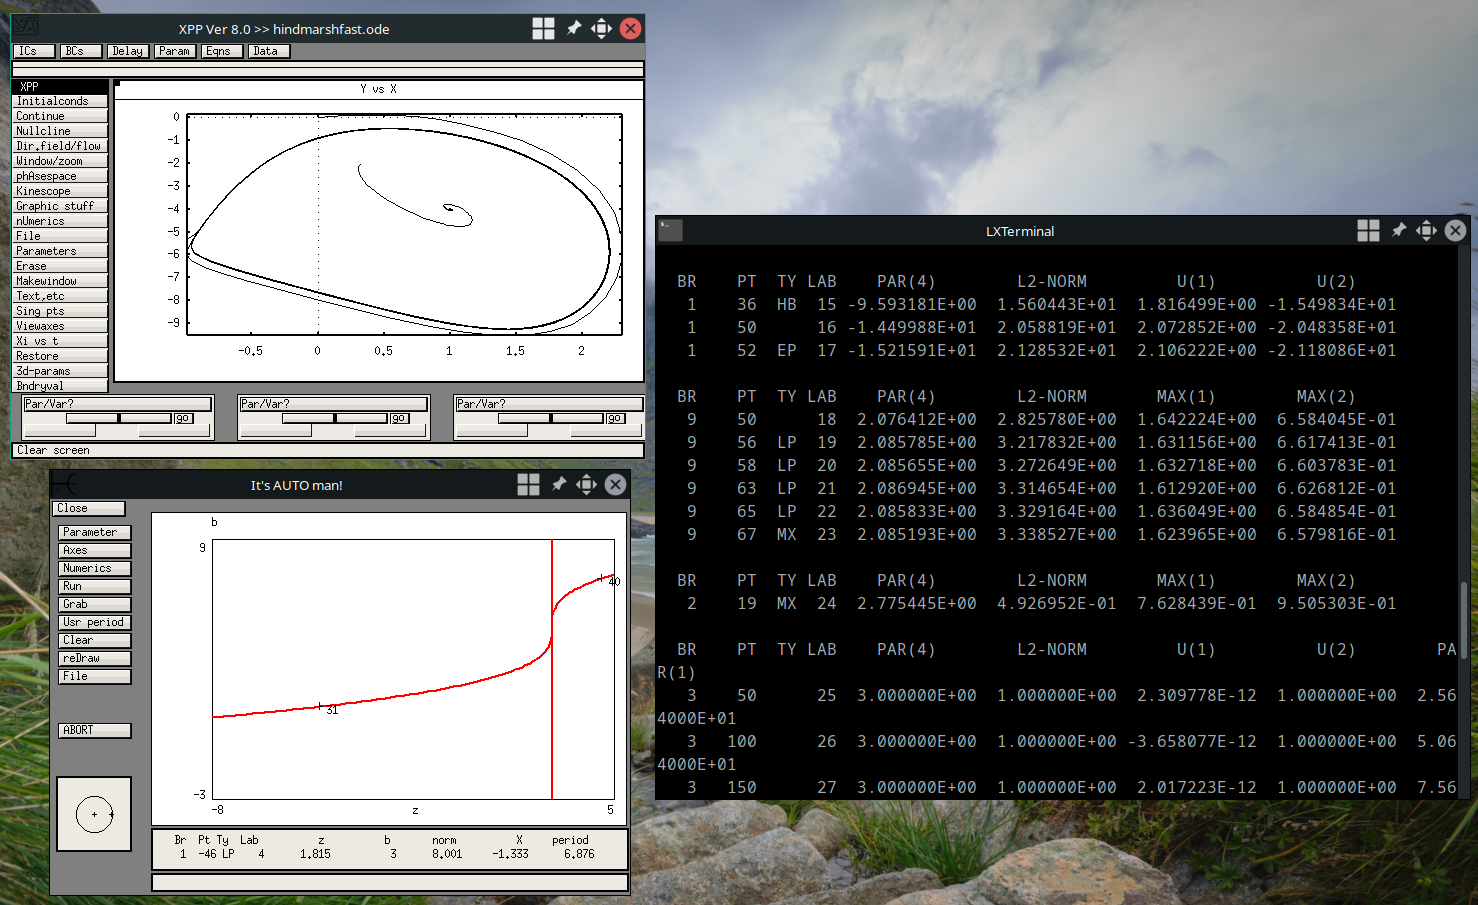
\includegraphics[height=.9\textheight]{auto3.png}
\end{center}
\end{frame}

\begin{frame}[label={sec:org218fa87}]{HR Bifurcations in MATCONT (again)}
\begin{center}
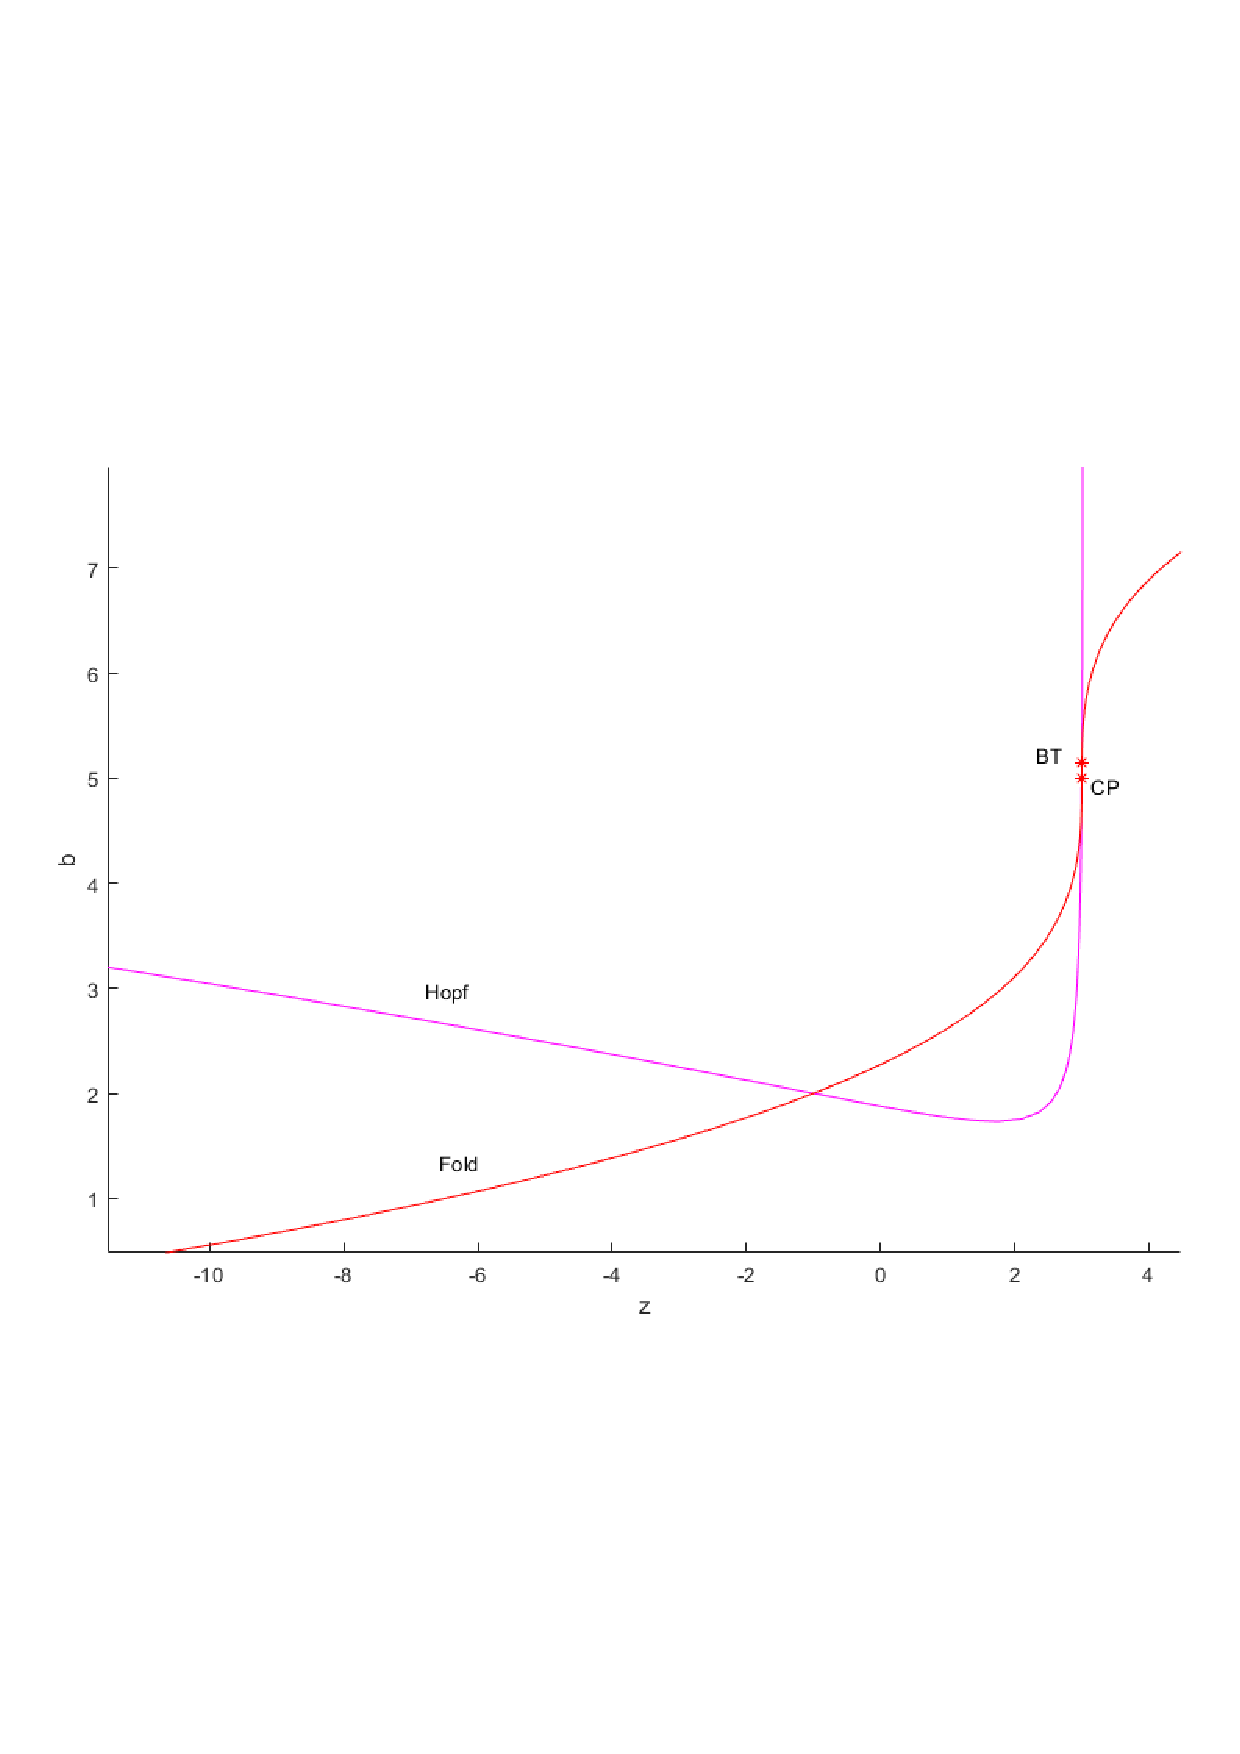
\includegraphics[trim={1cm 7cm 1cm 8cm}, clip,height=.9\textheight]{HRzbBif.pdf}
\end{center}
\end{frame}

\section{Next steps}
\label{sec:org7dfe0b0}
\begin{frame}[label={sec:org4f4551a}]{Next steps}
\begin{itemize}
\item Read more about the cubic Lienard model (some of the papers have a good discussion of bifurcation analysis)
\item Reproduce some of the bifurcation diagrams from the literature
\begin{itemize}
\item Repeat with each of the different continuation softwares I'm testing
\end{itemize}
\item Once I'm familiar with a software package, add it to the comparison paper
\item To study homoclinic bifurcations, or not to study homoclinic bifurcations?
\end{itemize}
\end{frame}
\end{document}
